
%% CLASS MANUAL FOUND IN http://blog.poormansmath.net/latex-class-for-lecture-notes/ %%
%% CLASS AUTHOR Stefano Maggiolo %%
\documentclass[english,course]{Notes}

\title{Network \& Operation Systems Essentials}
\subject{Computer Science}
\author{Joao Almeida-Domingues}
\email{2334590D@student.gla.ac.uk}
\speaker{Dr Nikos Ntarmos}
\date{24}{09}{2018}
\dateend{04}{12}{2019}
\place{University of Glasgow}


%%%%%%%%%%%%%%%%PACKAGES%%%%%%%%%%%%%%%%%%%%%%%%%%%%%

\usepackage[backend=biber, style=reading]{biblatex} %bibliography
\bibliography{} %add bib file name

\renewcommand{\abstractname}{\vspace{3\baselineskip}} %hack to remove abstract

\begin{document}


\begin{abstract}
\par{These lecture notes were collated by me from a mixture of sources , the two main sources being the lecture notes provided by the lecturer and the content presented in-lecture. All other referenced material (if used) can be found in the \ita{Bibliography} and \ita{References} sections.}
\par{The primary goal of these notes is to function as a succinct but comprehensive revision aid, hence if you came by them via a search engine , please note that they're not intended to be a reflection of the quality of the materials referenced or the content lectured.}
\par{Lastly, with regards to formatting, the pdf doc was typeset in \LaTeX , using a modified version of Stefano Maggiolo's \href{http://blog.poormansmath.net/latex-class-for-lecture-notes/}{\underline{\textcolor{blue}{class}}}}
\end{abstract}
\newpage


\section{Routing}
\subsection{Distance Vector Protocols}

\par{\textbf{Motivation} \\ Given that the internet is by definition a network of networks , which though connected does not have a central management system which can keep track of all nodes, how are routing paths known? What's the optimal path between any two nodes? \\}

\par{DVPs tackle this problem by assigning a vector to each node containing the distance to every other node in the network. The main idea here is that initially each node will have access to the \ita{cost} of sending a packet to its immediate neighbours. Then, once routing tables start being built, they are also shared amongst the nodes. Hence, farther away nodes costs are now known also via intermediary nodes. i.e if $A \rightarrow B$ and $B \rightarrow C$ then, once $B$ shares its routing table with $A, C$ it can now be known that $A \rightarrow B \rightarrow C$ . Eventually all nodes will converge towards a \ita{steady state}, where all tables have been computed}

\rem{The algorithm aims to find the shortest-cost path. Hence, routing tables can be updated at each \ita{``iteration''}, if a shortest path is found between any two nodes.}

\rem{Though it makes it easier to think of the process as occurring in rounds, where each round corresponds to 1-\ita{hop} in the network with all tables synced, this is not necessarily true}

\defn{Steady State}{when all  nodes have computing their routing tables}

\subsubsection{Algorithm}

\rem{During the process \ita{forwarding tables} are used as an intermediate step, where triplets of the type \texttt{[Destination, Cost, NextHop]} are shared so that each node can track who sent them the info.}

\begin{enumerate}
	\item Populate each node with the vector \texttt{[Cost , NextHop]}
	\item Share routing table 
	\item If routing tables received contain unknown nodes and/or cost to unknown is lower
	\begin{enumerate}
		\item Update vector cost \texttt{[DestCost + UnkCost , NextHop]}
	\end{enumerate}
	\item Repeat from 2 until all nodes are known and periodically (topology check)
\end{enumerate}

\rem{Note that if any link breaks, then the process need not be restarted in full. The linked nodes simply change their vector appropriately. The affected nodes then attempt to build alternative paths by the same process}

\par{This process is usually illustrated by a 2D table}

\example{

\IfFileExists{dvp}{}{\write18{wget https://cdn.mathpix.com/snip/images/gfpnAk7NlDjdqvW1Q4CxyGBgAsf9e5U4qjy3TCRuLiA.original.fullsize.png -O dvp.png}}
\begin{figure}[H]
\centering
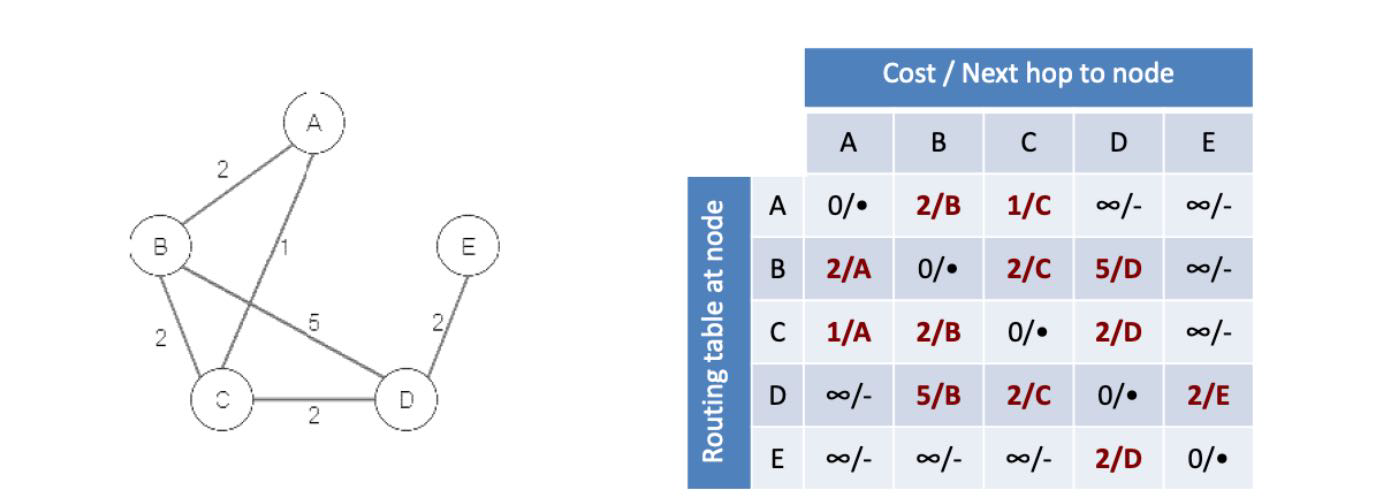
\includegraphics[width=0.5\textwidth]{dvp.png}
\end{figure}

\par{Take $A$ for example. We now see that it has access to $B,C$ tables. $B,C$ are both connected, but their cost does not improve upon $A$ costs to each. So $A_{B} , A_{C}$ remain unchanged. However, $A_{D}$ is currently unknown , but can be reached by both. Comparing their costs, we see that $A \rightarrow B \rightarrow D = 2 + 5$ and   $A \rightarrow C \rightarrow D = 1 + 2 = 3$ . Hence we update $A_{D} = [3,C]$ , which reads essentially as \ita{``A to D via C has  a total cost of $3$''}}

\todo{typeset tables \& adjust layout}
}

\subsubsection{Limitations}

\par{A major problem with DVP is \ita{count-to-infinity} . Due to asynchronicity, in particular in larger networks, a broken link can fail to be communicated to farther away nodes in time. This means that one of the nodes involved in the broken link $A,B$, say $B$ might receive an outdated table from another node $C$, before $C$ is updated by $B$ of the broken link . Hence, $C$ will update $B_{A}$ with the old path. At this point, $B$ will interpret this a new existing path to $A$ via $C$, adding the cost $BCA$. In the next round $C$ will see that $B$ has changed again, and will updated its cost appropriately, creating a feedback loop}

\par{Possible solutions:}

\begin{enumerate}
	\item Define $\infty$ , bounding the \#hops
	\item Split Horizon : prevents feedback loop by not advertising route back to the node which sent the update
\end{enumerate}

\par{Due to this, these protocols always suffer from slow convergence, since it tries to minimise state at nodes}

\subsubsection{Advantages}

\begin{enumerate}
	\item Simple to implement
	\item Info at each node is minimised $\implies$ faster computation times $O(n)$
	\item Good for small networks
\end{enumerate}

\subsection{Link State}

\par{It's composed of 2 main stages : \ita{Flooding} and \ita{Shortest Path Calculation}. The main difference here being that the shortest path computation is not done  locally once and then its result is transmitted to the neighbours, but instead nodes advertise information about all its neighbours and the link costs to them in the ad�vertisement step. Those very same packets are then re-broadcasted to each neighbour, until all nodes have received the entire map of the network. Packed with the full map, each node is then free to compute a centralised computation* of the shortest path from itself to any other node.}
\mymarginpar{*Usually by application of Djisktra's algorithm}


\defn{Flooding}{every incoming packet is rebroadcasted through each outgoing link}
\defn{Link State Information}{links to neighbours, and the cost of using those links}


\subsubsection{Limitations}

\begin{enumerate}
	\item Complex implementation
	\item Each node has to have a complete map of the network $\implies$ slower computation times $O(n^{2})$
\end{enumerate}

\subsubsection{Advantages}
\begin{enumerate}
	\item Fast convergence $\implies$ good for large networks
\end{enumerate}


\newpage
\nocite{*}
\printbibliography

\todos

\end{document}